\documentclass{standalone}
\usepackage{tikz}
\usetikzlibrary{patterns, positioning}

\begin{document}
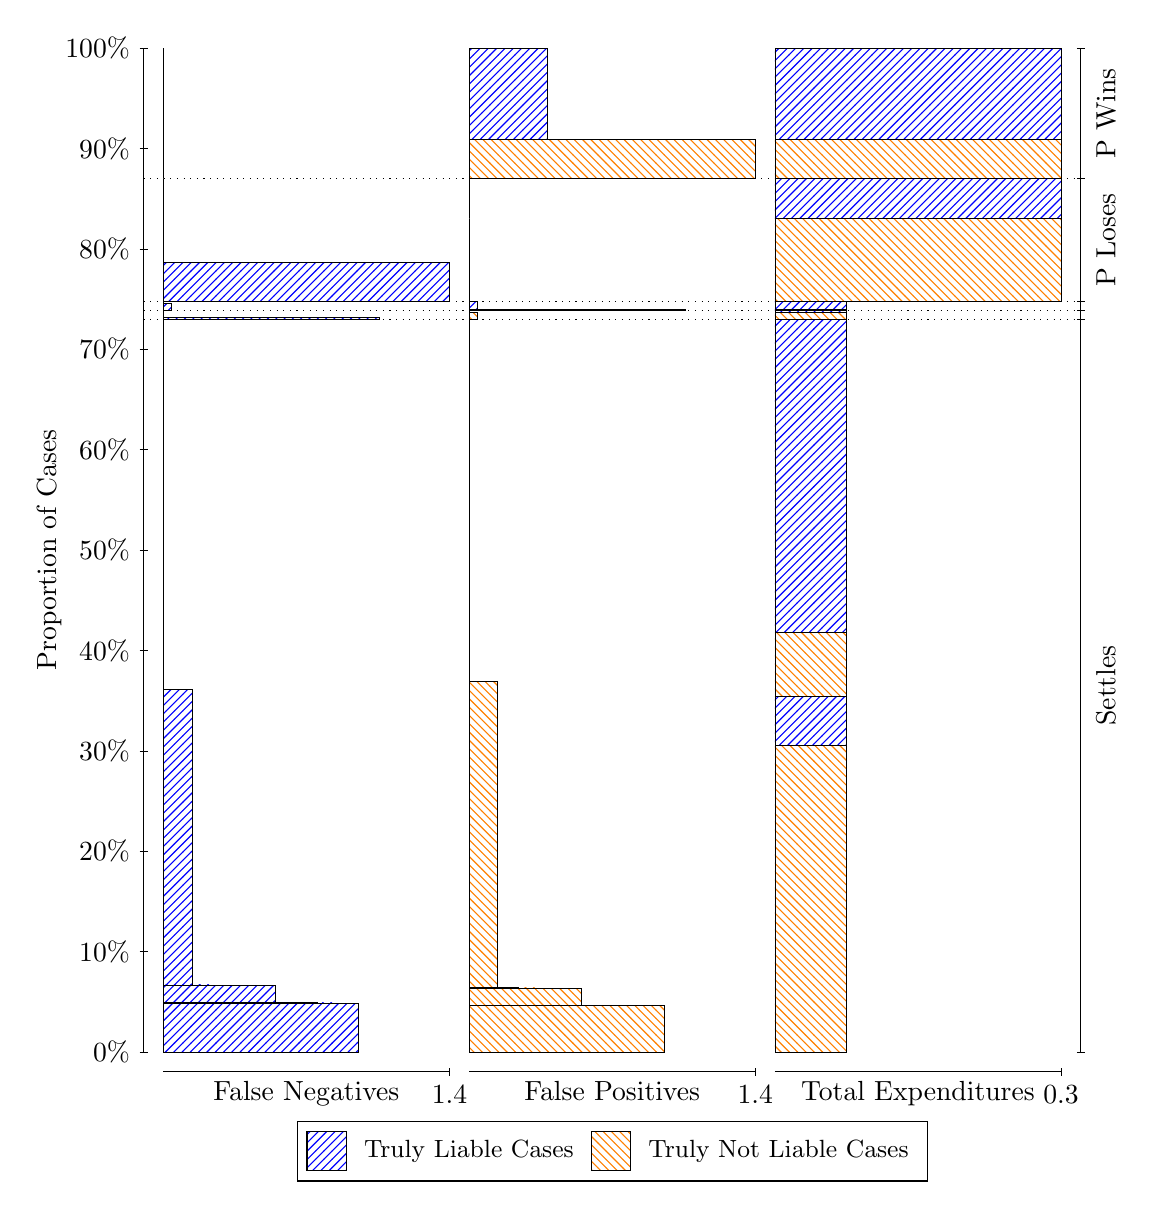
\begin{tikzpicture}
\draw[black, very thin] (1.5,1.75) -- (1.5,14.5);
\node[rotate=90, anchor=center] at (0.3, 8.125) {Proportion of Cases};
\draw[black, very thin] (1.45,1.75) -- (1.55,1.75);
\node[anchor=east] at (1.45, 1.75) {0\%};
\draw[black, very thin] (1.45,3.025) -- (1.55,3.025);
\node[anchor=east] at (1.45, 3.025) {10\%};
\draw[black, very thin] (1.45,4.3) -- (1.55,4.3);
\node[anchor=east] at (1.45, 4.3) {20\%};
\draw[black, very thin] (1.45,5.575) -- (1.55,5.575);
\node[anchor=east] at (1.45, 5.575) {30\%};
\draw[black, very thin] (1.45,6.85) -- (1.55,6.85);
\node[anchor=east] at (1.45, 6.85) {40\%};
\draw[black, very thin] (1.45,8.125) -- (1.55,8.125);
\node[anchor=east] at (1.45, 8.125) {50\%};
\draw[black, very thin] (1.45,9.4) -- (1.55,9.4);
\node[anchor=east] at (1.45, 9.4) {60\%};
\draw[black, very thin] (1.45,10.675) -- (1.55,10.675);
\node[anchor=east] at (1.45, 10.675) {70\%};
\draw[black, very thin] (1.45,11.95) -- (1.55,11.95);
\node[anchor=east] at (1.45, 11.95) {80\%};
\draw[black, very thin] (1.45,13.225) -- (1.55,13.225);
\node[anchor=east] at (1.45, 13.225) {90\%};
\draw[black, very thin] (1.45,14.5) -- (1.55,14.5);
\node[anchor=east] at (1.45, 14.5) {100\%};

\draw[black, very thin] (13.4,1.75) -- (13.4,14.5);
\draw[black, very thin] (13.35,1.75) -- (13.45,1.75);
\node[anchor=west] at (13.35, 1.75) {};
\draw[black, very thin] (13.35,11.056) -- (13.45,11.056);
\node[anchor=west] at (13.35, 11.056) {};
\draw[black, very thin] (13.35,11.164) -- (13.45,11.164);
\node[anchor=west] at (13.35, 11.164) {};
\draw[black, very thin] (13.35,11.279) -- (13.45,11.279);
\node[anchor=west] at (13.35, 11.279) {};
\draw[black, very thin] (13.35,12.84) -- (13.45,12.84);
\node[anchor=west] at (13.35, 12.84) {};
\draw[black, very thin] (13.35,14.5) -- (13.45,14.5);
\node[anchor=west] at (13.35, 14.5) {};

\draw[black, very thin, pattern color=blue, pattern=north east lines] (1.75,1.75) rectangle (4.2273,2.37);
\draw[black, very thin, pattern color=blue, pattern=north east lines] (1.75,2.37) rectangle (3.963,2.3745);
\draw[black, very thin, pattern color=blue, pattern=north east lines] (1.75,2.3745) rectangle (3.6988,2.3792);
\draw[black, very thin, pattern color=blue, pattern=north east lines] (1.75,2.3792) rectangle (3.4345,2.3842);
\draw[black, very thin, pattern color=blue, pattern=north east lines] (1.75,2.3842) rectangle (3.1703,2.5959);
\draw[black, very thin, pattern color=blue, pattern=north east lines] (1.75,2.5959) rectangle (2.9061,2.598);
\draw[black, very thin, pattern color=blue, pattern=north east lines] (1.75,2.598) rectangle (2.6418,2.6001);
\draw[black, very thin, pattern color=blue, pattern=north east lines] (1.75,2.6001) rectangle (2.3776,2.6023);
\draw[black, very thin, pattern color=blue, pattern=north east lines] (1.75,2.6023) rectangle (2.1133,6.3519);
\draw[black, very thin, pattern color=orange, pattern=north west lines] (1.75,6.3519) rectangle (1.75,11.056);
\draw[black, very thin, pattern color=blue, pattern=north east lines] (1.75,11.056) rectangle (4.4915,11.076);
\draw[black, very thin, pattern color=orange, pattern=north west lines] (1.75,11.076) rectangle (1.75,11.164);
\draw[black, very thin, pattern color=blue, pattern=north east lines] (1.75,11.164) rectangle (1.8491,11.258);
\draw[black, very thin, pattern color=orange, pattern=north west lines] (1.75,11.258) rectangle (1.75,11.279);
\draw[black, very thin, pattern color=blue, pattern=north east lines] (1.75,11.279) rectangle (5.3833,11.782);
\draw[black, very thin, pattern color=orange, pattern=north west lines] (1.75,11.782) rectangle (1.75,12.84);
\draw[black, very thin, pattern color=orange, pattern=north west lines] (1.75,12.84) rectangle (1.75,13.344);
\draw[black, very thin, pattern color=blue, pattern=north east lines] (1.75,13.344) rectangle (1.75,14.5);
\draw[black, very thin, pattern color=orange, pattern=north west lines] (5.6333,1.75) rectangle (8.1106,2.3386);
\draw[black, very thin, pattern color=orange, pattern=north west lines] (5.6333,2.3386) rectangle (7.8464,2.3404);
\draw[black, very thin, pattern color=orange, pattern=north west lines] (5.6333,2.3404) rectangle (7.5821,2.3422);
\draw[black, very thin, pattern color=orange, pattern=north west lines] (5.6333,2.3422) rectangle (7.3179,2.3438);
\draw[black, very thin, pattern color=orange, pattern=north west lines] (5.6333,2.3438) rectangle (7.0536,2.5532);
\draw[black, very thin, pattern color=orange, pattern=north west lines] (5.6333,2.5532) rectangle (6.7894,2.5532);
\draw[black, very thin, pattern color=orange, pattern=north west lines] (5.6333,2.5532) rectangle (6.7894,2.5592);
\draw[black, very thin, pattern color=orange, pattern=north west lines] (5.6333,2.5592) rectangle (6.5252,2.565);
\draw[black, very thin, pattern color=orange, pattern=north west lines] (5.6333,2.565) rectangle (6.2609,2.5704);
\draw[black, very thin, pattern color=orange, pattern=north west lines] (5.6333,2.5704) rectangle (5.9967,6.4542);
\draw[black, very thin, pattern color=blue, pattern=north east lines] (5.6333,6.4542) rectangle (5.6333,11.056);
\draw[black, very thin, pattern color=orange, pattern=north west lines] (5.6333,11.056) rectangle (5.7324,11.145);
\draw[black, very thin, pattern color=blue, pattern=north east lines] (5.6333,11.145) rectangle (5.6333,11.164);
\draw[black, very thin, pattern color=orange, pattern=north west lines] (5.6333,11.164) rectangle (8.3748,11.185);
\draw[black, very thin, pattern color=blue, pattern=north east lines] (5.6333,11.185) rectangle (5.7324,11.279);
\draw[black, very thin, pattern color=orange, pattern=north west lines] (5.6333,11.279) rectangle (5.6333,12.337);
\draw[black, very thin, pattern color=blue, pattern=north east lines] (5.6333,12.337) rectangle (5.6333,12.84);
\draw[black, very thin, pattern color=orange, pattern=north west lines] (5.6333,12.84) rectangle (9.2667,13.344);
\draw[black, very thin, pattern color=blue, pattern=north east lines] (5.6333,13.344) rectangle (6.6242,14.5);
\draw[black, very thin, pattern color=orange, pattern=north west lines] (9.5167,1.75) rectangle (10.425,5.6392);
\draw[black, very thin, pattern color=blue, pattern=north east lines] (9.5167,5.6392) rectangle (10.425,6.2637);
\draw[black, very thin, pattern color=orange, pattern=north west lines] (9.5167,6.2637) rectangle (10.425,7.0787);
\draw[black, very thin, pattern color=blue, pattern=north east lines] (9.5167,7.0787) rectangle (10.425,11.056);
\draw[black, very thin, pattern color=orange, pattern=north west lines] (9.5167,11.056) rectangle (10.425,11.145);
\draw[black, very thin, pattern color=blue, pattern=north east lines] (9.5167,11.145) rectangle (10.425,11.164);
\draw[black, very thin, pattern color=orange, pattern=north west lines] (9.5167,11.164) rectangle (10.425,11.185);
\draw[black, very thin, pattern color=blue, pattern=north east lines] (9.5167,11.185) rectangle (10.425,11.279);
\draw[black, very thin, pattern color=orange, pattern=north west lines] (9.5167,11.279) rectangle (13.15,12.337);
\draw[black, very thin, pattern color=blue, pattern=north east lines] (9.5167,12.337) rectangle (13.15,12.84);
\draw[black, very thin, pattern color=orange, pattern=north west lines] (9.5167,12.84) rectangle (13.15,13.344);
\draw[black, very thin, pattern color=blue, pattern=north east lines] (9.5167,13.344) rectangle (13.15,14.5);
\draw[black, dotted] (1.5,11.056) -- (13.4,11.056);
\draw[black, dotted] (1.5,11.164) -- (13.4,11.164);
\draw[black, dotted] (1.5,11.279) -- (13.4,11.279);
\draw[black, dotted] (1.5,12.84) -- (13.4,12.84);
\draw[black, very thin] (1.75,1.5) -- (5.3833,1.5);
\node[anchor=north] at (3.5667, 1.5) {False Negatives};
\draw[black, very thin] (5.3833,1.45) -- (5.3833,1.55);
\node[anchor=north] at (5.3833, 1.45) {1.4};

\draw[black, very thin] (5.6333,1.5) -- (9.2667,1.5);
\node[anchor=north] at (7.45, 1.5) {False Positives};
\draw[black, very thin] (9.2667,1.45) -- (9.2667,1.55);
\node[anchor=north] at (9.2667, 1.45) {1.4};

\draw[black, very thin] (9.5167,1.5) -- (13.15,1.5);
\node[anchor=north] at (11.333, 1.5) {Total Expenditures};
\draw[black, very thin] (13.15,1.45) -- (13.15,1.55);
\node[anchor=north] at (13.15, 1.45) {0.3};

\node[black, centered, rotate=90] at (13.72, 6.403) {Settles};


\node[black, centered, rotate=90] at (13.72, 12.06) {P Loses};
\node[black, centered, rotate=90] at (13.72, 13.67) {P Wins};

\draw (7.449999999999999,1.5) node[draw=none] (baseCoordinate) {};
\begin{scope}[align=center]
        \matrix[scale=0.5, draw=black, below=0.5cm of baseCoordinate, nodes={draw}, column sep=0.1cm]{
            \node[rectangle, draw, minimum width=0.5cm, minimum height=0.5cm, pattern=north east lines, pattern color=blue] {}; &
            \node[draw=none, font=\small] (B) {Truly Liable Cases}; &
            \node[rectangle, draw, minimum width=0.5cm, minimum height=0.5cm, pattern=north west lines, pattern color=orange] {}; &
            \node[draw=none, font=\small] (B) {Truly Not Liable Cases}; \\
            };
\end{scope}

\end{tikzpicture}
\end{document}